\subsection{Components of RAVEN}
\label{sub:InputComponents}
The RAVEN code does not have a fixed calculation flow, since all of its basic
objects can be combined in order to create a user-defined calculation flow.
%
Thus, its input, eXtensible Markup Language (XML) format, is organized in different XML blocks, each with a
different functionality. For more information about XML, please click on the link:
\href{https://www.w3schools.com/xml/default.asp}{\textbf{XML tutorial}}.
%
\\The main input blocks are as follows:
\begin{itemize}
  \item \xmlNode{Simulation}: The root node containing the
  entire input, all of
  the following blocks fit inside the \emph{Simulation} block.
  %
  \item \xmlNode{RunInfo}: Specifies the calculation
  settings (number of parallel simulations, etc.).
  %
  \item \xmlNode{Files}: Specifies the files to be
  used in the calculation.
  %
  \item \xmlNode{Distributions}: Defines distributions
  needed for describing parameters, etc.
  %
  \item \xmlNode{Samplers}: Sets up the strategies used for
  exploring an uncertain domain.
  %
  \item \xmlNode{DataObjects}: Specifies internal data objects
  used by RAVEN.
  %
  \item \xmlNode{Databases}: Lists the HDF5 databases used
  as input/output to a
  RAVEN run.
  %
  \item \xmlNode{OutStreams}: Visualization and
  Printing system block.
  %
  \item \xmlNode{Models}: Specifies codes, ROMs,
  post-processing analysis, etc.
  %
  \item \xmlNode{Functions}: Details interfaces to external
  user-defined functions and modules the user will be building and/or running.
  %
  \item \xmlNode{VariableGroups}: Creates a collection of variables.
  %
  \item \xmlNode{Optimizers}: Performs the driving of a specific goal function over
  the model for value optimization.
  %
  \item \xmlNode{Metrics}: Calculate the distance values among points and histories.
  %
  \item \xmlNode{Steps}: Combines other blocks to detail a
  step in the RAVEN workflow including I/O and computations to be performed.
  %
\end{itemize}

Each of these components are explained in dedicated sections of the user manual ~\cite{RAVENuserManual}, and can
be used as building blocks to construct certain calculation flow, as shown in Figure.~\ref{fig:ravenStructure}.
In this guide, we will only show how to use these components to build the analysis flow, and we recommend the user
to check the user manual ~\cite{RAVENuserManual} for the detailed descriptions.

\begin{figure}[h!]
  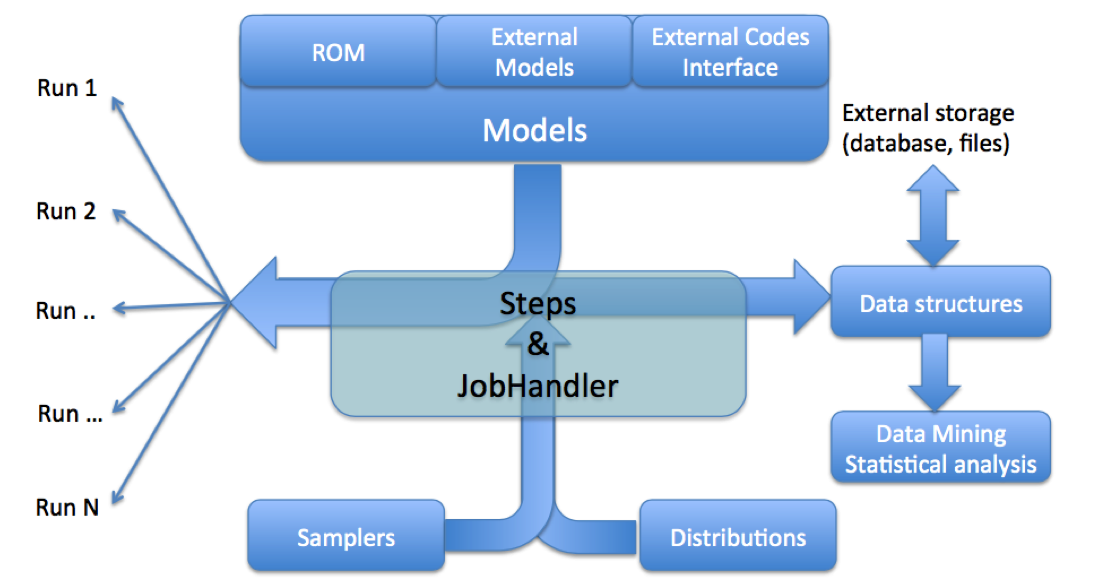
\includegraphics[width=\textwidth]{pics/ravenStructure.png}
  \caption{RAVEN structures}
  \label{fig:ravenStructure}
\end{figure}

In addition, RAVEN allows the user to load any external input file that contains the required XML nodes into the RAVEN main input
file, and provide the standard XML comments, using\verb|<!--| and \verb|-->|. For example, one can use the following template to load
the \xmlNode{Distributions} from file `Distributions.xml'.
%
\begin{lstlisting}[style=XML,morekeywords={node,xmlToLoad}]
<Simulation verbosity='all'>
  ...
  <!-- An Example Comment -->
  <Steps verbosity='debug'>
    ...
  </Steps>
  ...
  <ExternalXML node='Distributions' xmlToLoad='path_to_folder/Distributions.xml'/>
  ...
</Simulation>
\end{lstlisting}
%
RAVEN also allows the user to control the level of output to the user interface by using \xmlAttr{verbosity} system. These settings can be
declared globally as attributes in the \xmlNode{Simulation} node, or locally in each block node as shown in above template.
The verbosity levels are
\begin{itemize}
\item \xmlString{silent} - Only simulation-breaking errors are displayed.
\item \xmlString{quiet} - Errors as well as warnings are displayed.
\item \xmlString{all} (default) - Errors, warnings, and messages are displayed.
\item \xmlString{debug} - For developers. All errors, warnings, messages, and debug messages are displayed.
\end{itemize}

